%  LaTeX support: latex@mdpi.com 
%  In case you need support, please attach all files 
%  that are necessary for compiling as well as the log file, 
%  and specify the details of your LaTeX setup 
%  (which operating system and LaTeX version / tools you are using).

%=================================================================
\documentclass[ijgi,article,submit,moreauthors,pdftex]{Definitions/mdpi} 


%=================================================================
\firstpage{1} 
\makeatletter 
\setcounter{page}{\@firstpage} 
\makeatother
\pubvolume{xx}
\issuenum{1}
\articlenumber{5}
\pubyear{2019}
\copyrightyear{2019}
%\externaleditor{Academic Editor: name}
\history{Received: date; Accepted: date; Published: date}
%\updates{yes} % If there is an update available, un-comment this line

%% MDPI internal command: uncomment if new journal that already uses continuous page numbers 
%\continuouspages{yes}

%------------------------------------------------------------------
% The following line should be uncommented if the LaTeX file is uploaded to arXiv.org
%\pdfoutput=1

%=================================================================
% Add packages and commands here. The following packages are loaded in our class file: fontenc, calc, indentfirst, fancyhdr, graphicx, lastpage, ifthen, lineno, float, amsmath, setspace, enumitem, mathpazo, booktabs, titlesec, etoolbox, amsthm, hyphenat, natbib, hyperref, footmisc, geometry, caption, url, mdframed, tabto, soul, multirow, microtype, tikz

\usepackage{xspace}


%=================================================================
%% Please use the following mathematics environments: Theorem, Lemma, Corollary, Proposition, Characterization, Property, Problem, Example, ExamplesandDefinitions, Hypothesis, Remark, Definition, Notation, Assumption
%% For proofs, please use the proof environment (the amsthm package is loaded by the MDPI class).




\graphicspath{{images/}}

\newcommand{\Astar}{A$^{\!\star}$\xspace}

\newcommand{\e}[1]{\times 10^{#1}}
\newcommand{\fig}{Figure~}
\newcommand{\eq}{Equation~}
\newcommand{\fo}{Formula~}
\newcommand{\sect}{Section~}
\newcommand{\mytable}{Table~}
\newcommand{\chap}{Chapter~}
\newcommand{\figs}{Figures~}
\newcommand{\eqs}{Equations~}
\newcommand{\fos}{Formulas~}
\newcommand{\sects}{Sections~}
\newcommand{\tabs}{Tables~}
\newcommand{\chaps}{Chapters~}


%=================================================================
% Full title of the paper (Capitalized)
\Title{Paralleling Generalization Operations to Support Smooth Zooming:
Case Study of Merging Land-Cover Parcels}
%\Title{Merging land-cover parcels parallelly 
%to support smooth zooming of web maps}

% Author Orchid ID: enter ID or remove command
\newcommand{\orcidauthorA}{0000-0000-000-000X} % Add \orcidA{} behind the author's name
%\newcommand{\orcidauthorB}{0000-0000-000-000X} % Add \orcidB{} behind the author's name

% Authors, for the paper (add full first names)
\Author{
Firstname Lastname $^{1,\dagger,\ddagger}$\orcidA{}, 
Firstname Lastname $^{1,\ddagger}$ and 
Firstname Lastname $^{2,}$*}

% Authors, for metadata in PDF
\AuthorNames{Firstname Lastname, Firstname Lastname and Firstname Lastname}

% Affiliations / Addresses (Add [1] after \address if there is only one affiliation.)
\address{%
$^{1}$ \quad Affiliation 1; e-mail@e-mail.com\\
$^{2}$ \quad Affiliation 2; e-mail@e-mail.com}

% Contact information of the corresponding author
\corres{Correspondence: e-mail@e-mail.com; Tel.: (optional; include country code; 
if there are multiple corresponding authors, add author initials) +xx-xxxx-xxx-xxxx (F.L.)}

% Current address and/or shared authorship
\firstnote{Current address: Affiliation 3} 
\secondnote{These authors contributed equally to this work.}
% The commands \thirdnote{} till \eighthnote{} are available for further notes

%\simplesumm{} % Simple summary

%\conference{} % An extended version of a conference paper

% Abstract (Do not insert blank lines, i.e. \\) 
\abstract{
%meaning of time.
Land-cover parcels are important features on maps.
When users zoom out on digital maps, 
some land-cover parcels become too tiny to be seen, 
which result in visual clutters. 
To avoid this problem, 
we merge small parcels into their neighbors to form larger parcels. 
We define an \emph{event} as merging a small parcel into a neighbor 
(where the neighbor gradually expands over the small parcel).
However, because of the given sequence 
in which the events are processed one by one, 
the map users still experience many small shock changes 
(because the merging transition time of their zooming out can be short).
We try to produce more-smooth changes by paralleling the events.
We define a \emph{step} as a set of merging events happening at the same time.
In our method, a merging step is completely processed 
before the next merging step takes place (all sequential). 
In this way, each event has more time to be observed by users,
resulting in more smooth zooming. 
Furthermore, we require that 
all the pairs of parcels involved in the merging events of a step 
do not have any common neighbors, 
which makes the merging events independent from each other.
There are two benefits of this independency.
First, it is easy for us to maintain the topology of the map.
Second, users can more easily understand the events 
than merging several parcels into a single one.
This paper shows the details of finding and processing parallel events.
Then, this paper compares between the scale transitions of maps generated
based on single-event merging step and parallel-event merging step.
Our original contribution is the proposal of the parallel generalization
maintaining map consistency over scale change. 
%why? how? what? so what?
}

% Keywords
\keyword{Map generalization, Vario-scale maps, Continuous generalization}



%%%%%%%%%%%%%%%%%%%%%%%%%%%%%%%%%%%%%%%%%%
% Only for the journal Data:
%\dataset{DOI number or link to the deposited data set in cases where the data set is published or set to be published separately. If the data set is submitted and will be published as a supplement to this paper in the journal Data, this field will be filled by the editors of the journal. In this case, please make sure to submit the data set as a supplement when entering your manuscript into our manuscript editorial system.}

%\datasetlicense{license under which the data set is made available (CC0, CC-BY, CC-BY-SA, CC-BY-NC, etc.)}



%\setcounter{secnumdepth}{4}
%%%%%%%%%%%%%%%%%%%%%%%%%%%%%%%%%%%%%%%%%%
\begin{document}
%%%%%%%%%%%%%%%%%%%%%%%%%%%%%%%%%%%%%%%%%%



\section{Introduction}

When map users are reading digital maps,
they expect different levels of detail (LoDs) depending on scale.
For example, they may want to see individual buildings when zooming in
and see built-up areas when zooming out.
That is why geographical information is dependent on the scale
\citep{Muller1995Generalization,Weibel1997}. 
In order to prepare map data for different scales,
map generalization is used to generate coarser data 
for maps at smaller scales,
from a detailed map.
A lot of research has been devoted to map generalization.
\citet{Mackaness2017Generalization} gave a taxonomy of 
generalization algorithms, 
including selection, simplification, aggregation, and so on.
Often, a multi-representation database (MRDB) is used to store
maps at different scales and to send proper data to clients on request
\citep[\eg][]{Hampe2004multiple}.
However, large discrete changes between different map representations
may confuse users,
so continuous map generalization (CMG) is needed to
provide smooth scale zoom.
Algorithms of CMG have been proposed 
to morph raster maps
\citep[\eg][]{Pantazis2009a,Pantazis2009b}, 
to morph polylines
\citep[\eg][]{Noellenburg2008,Peng2013LSA,Deng2015,Li2017Annealing},
to generalize buildings
\citep[\eg][]{Li2017_Building,Peng2017Building,Touya2017Progressive},
to transform road networks
\citep[\eg][]{Suba2016Road,Chimani2014Eat},
and to transform administrative boundaries
\citep[\eg][]{Peng2016Admin}.
%Indeed, there are already many algorithms 
%for continuous map generalization.
%To adapt them into a web environment still needs a lot of effort.
%This paper contributes to merging land-cover parcels 
%in a web environment. 


Land-cover parcels are important on maps. 
When users zoom out,
some land-cover parcels become too tiny to be seen,
which result in visual clutter.
The clutter can be avoided by merging those tiny parcels 
with their neighbors.
For example, \citet{haunert2008f} developed a method based on
mixed-integer programming to merge land-cover parcels
for a map at a certain scale.
However, if zooming is realized by switching between
some levels of map representations, 
large and discrete changes usually happen
(e.g., from \fig\ref{fig:intro}a to \fig\ref{fig:intro}b), 
which is difficult for map users to understand.
To provide small changes, 
\citet{vanOosterom2005} proposed 
the topological Generalized Area Partitioning (tGAP) tree,
where at each step a single parcel is merged into
its most compatible neighbor 
(see \fig\ref{fig:intro}c--g).
Further, a space-scale cube (SSC) can be built so that 
map users can view the gradual transition of the merge operation
by slicing the SSC \citep[see][]{Meijers2020Web}.
This gradual strategy apparently allows users 
to follow the zooming more easily.


\begin{figure}[tb]
\centering
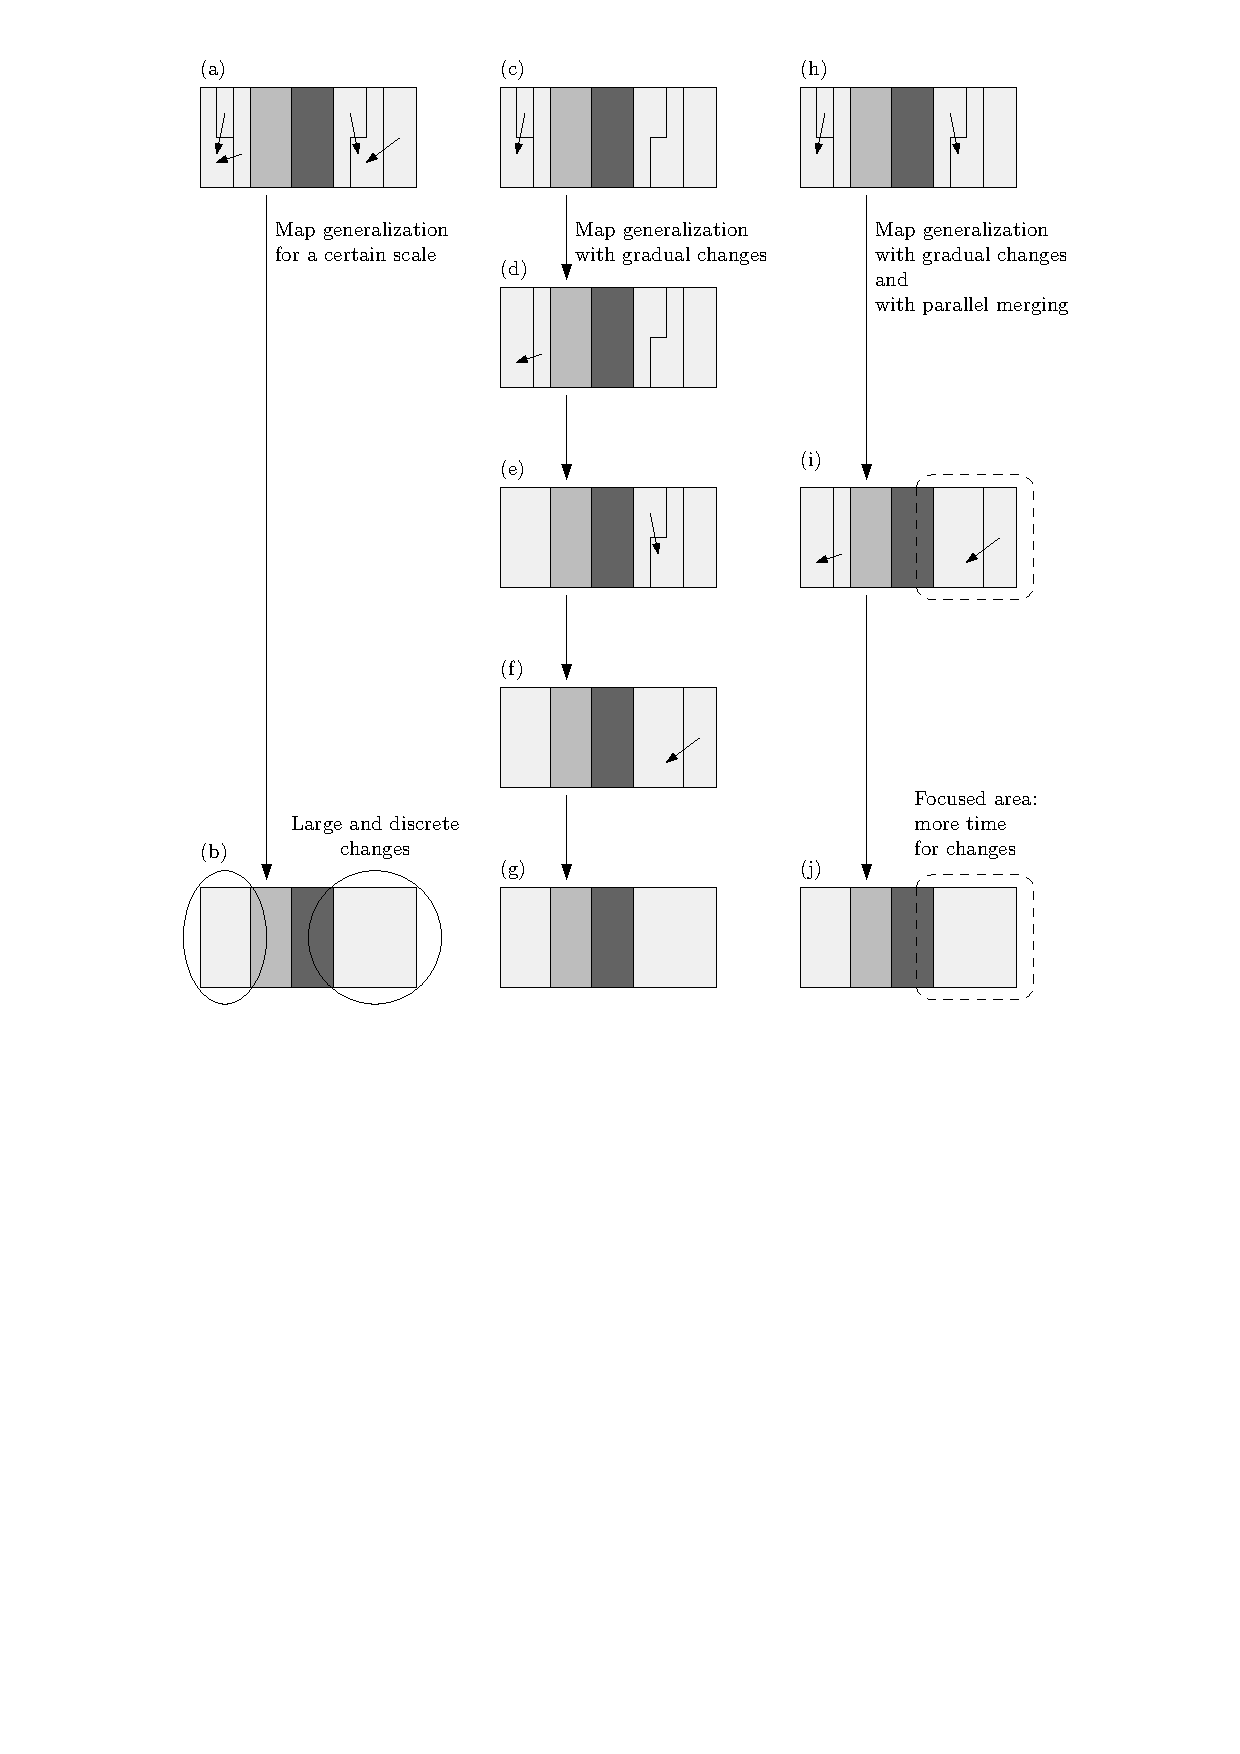
\includegraphics[page=1]{introduction}
\caption{A comparison of traditional map generalization (a--b),
map generalization with gradual changes (c--g),
and map generalization with parallel merging (h--j).
The ellipses show the places where large and discrete changes happen.
The dashed polygons show the place where a user may focus;
in the place, the user has twice of the time to perceive the merging
comparing to the merging of figures e--g.
Each arrow indicates that a parcel will be merged into another one. 
}
\label{fig:intro}
\end{figure}

When users zoom on maps, 
they do not want to wait for too long 
to see the desired level.
On a real map, however, 
there are way too many pairs of parcels to merge 
when users are zooming out.
If the pairs are processed one by one 
(e.g., \fig\ref{fig:intro}c--f),
then the time interval for each merging operation has to be very short.
For example, a user may still get the impression of
a shock change from \fig\ref{fig:intro}e to \fig\ref{fig:intro}g
even when the three parcels on the right-hand side of \fig\ref{fig:intro}e
are merged gradually.
To provide users with more gradual impression, 
we parallel the merging operations
(see \fig\ref{fig:intro}h--j).
If we select some of the merging operations
fairly evenly distributed on the whole map 
(there may be only a small number of merging operations 
happening on the screen),
then the changes are easy for users to understand
because these changes now have more time to take place.
For example, in the focused area, there is only one merging operation 
from \fig\ref{fig:intro}i to \fig\ref{fig:intro}j
while there are two merging operations  
from \fig\ref{fig:intro}e to \fig\ref{fig:intro}g;
a user has twice of the time to perceive the changes of the former,
comparing to the latter.

This paper is organized as follows.
\sect\ref{sec:realted_work} reviews some related work.
Our methodology is presented in \sect\ref{sec:methodology}.
We show a case study in \sect\ref{sec:case_study}.
Finally, \sect\ref{sec:concluding_remarks} draws our conclusion
and indicate our future work.





 
\section{Related Work}
\label{sec:realted_work}

\citet{vanOosterom2005} proposed a greedy algorithm 
to merge land-cover parcels one by one.
In each iteration, that algorithm takes the least important parcel and 
merges it into the most compatible neighbor.
The importance of a parcel is defined 
based on both the size and the type of the parcel.
The compatibility between a pair of parcels is defined based on 
both the length of the common boundary and the similarity of the types 
of the pair of parcels. 
\citet[\chap2]{Peng2019Thesis} tried to find an optimal sequence 
to merge land-cover parcels
based on the \Astar algorithm or an integer linear program.
A comparison to a greedy algorithm showed that 
the \Astar algorithm improves the quality of the merging sequences
in the sense of the type changes and the compactnesses of the parcels.
\citet{vanOosterom2014Support} pointed out that sequentially merging
land-cover parcels may result in a suboptimal smooth-zoom effect.
To provide better visualization, they suggested that
the merging operations should be paralleled.
Then, one question is how many operations 
should be paralleled for a given scale.
\citet{Thiemann2018LandCover} proposed a chain of operators 
to generalize a land-cover map.
In the chain of processing land-cover polygons, 
they integrated cleaning, dissolving, splitting, aggregating, reclassifying, and simplifying. 


\citet{Meijers2020Web} explained the principles of 
implementing a web map of land-cover parcels.
First, they generated an SSC, 
where a parcel on map becomes a polyhedron in the SSC.
They used the SSC because 
they wanted the web map to support smooth zoom
\citep[see][]{vanOosterom2014Support}.
Second, they showed how to slice the SSC 
to output a web map at a given scale.
The slicing is based on the GPU at the client side.
Third, they made chunks of the SSC 
so that they were able to send only the data of the place
where a map user was reading.
\citet{Suba2014Merge} proposed three methods 
to merge a pair of parcels in the manner of gradual change, 
which are the ``Single flat plane'', the ``Zipper'', and the ``Eater''.
Basically, the \emph{winner} gradually expands over the \emph{loser}.
We will use the ``Eater'' because it works for all kinds of polygons 
while the other two methods have limitation 
in terms of the type of a polygon.
For example, the two other methods do not work for some concave polygons.
\citet{Suba2016Road} continuously generalized a planar map of road network.
At each step, they process the least-important face.
Taking into account the condition of the face,
they put it back with higher importance, collapse it, 
or merge it into an adjacent face.
In addition to the generalization, 
they also observed the number of faces,
the area of faces, the number of road faces, the number of road edges,
and the number of operations (merge and split) 
when the scale of the map is decreasing.
These statistics can be good indications 
for (continuous) map generalization.
\citet{Huang2016Webmap} pointed out that
the effort of implementing online maps 
had been spent mainly on preparing data on the server side.
They studied the communication of map data 
between the server side and the client side.
They proposed different strategies of assigning 
the work of handling map data
according to the machine abilities of the clients.

\citet{Huang2017Matrix} used a matrix to guide 
both pruning rivers and removing vertices for a river network, 
where the rows and the columns respectively represent
the rivers and the vertices.
According to the matrix, 
they were able to decide which rivers and vertices 
should be remained for a given scale.
To this purpose, they proposed a method 
to compute how many rivers and vertices 
should be kept according to that given scale.






%\citet{Thiemann2018LandCover}
%\citet{Dumont2020MultiScale}
%\citet{Meijers2015Parallel}

%

\section{Methodology}
\label{sec:methodology}

%UML?
%Flowchart of the framework?



We define an \emph{event} as a single generalization operation, 
such as merging a small parcel into a neighbor.
For example, \fig\ref{fig:event_and_step}b is obtained from 
\fig\ref{fig:event_and_step}a by processing one merging event,
where the dashed polygon marks the new parcel from the merging.
Similarly, \fig\ref{fig:event_and_step}c is obtained from 
\fig\ref{fig:event_and_step}a by processing two merging events.
We define a \emph{step} as 
a set of events happening at the same time.
For example, 
\fig\ref{fig:event_and_step}b is obtained from 
\fig\ref{fig:event_and_step}a by processing merging step with one event.
\fig\ref{fig:event_and_step}d is obtained from 
\fig\ref{fig:event_and_step}c by processing merging step with two events.
In our method, a merging step is completely processed 
before the next step takes place (all sequential). 

\begin{figure}[tb]
\centering
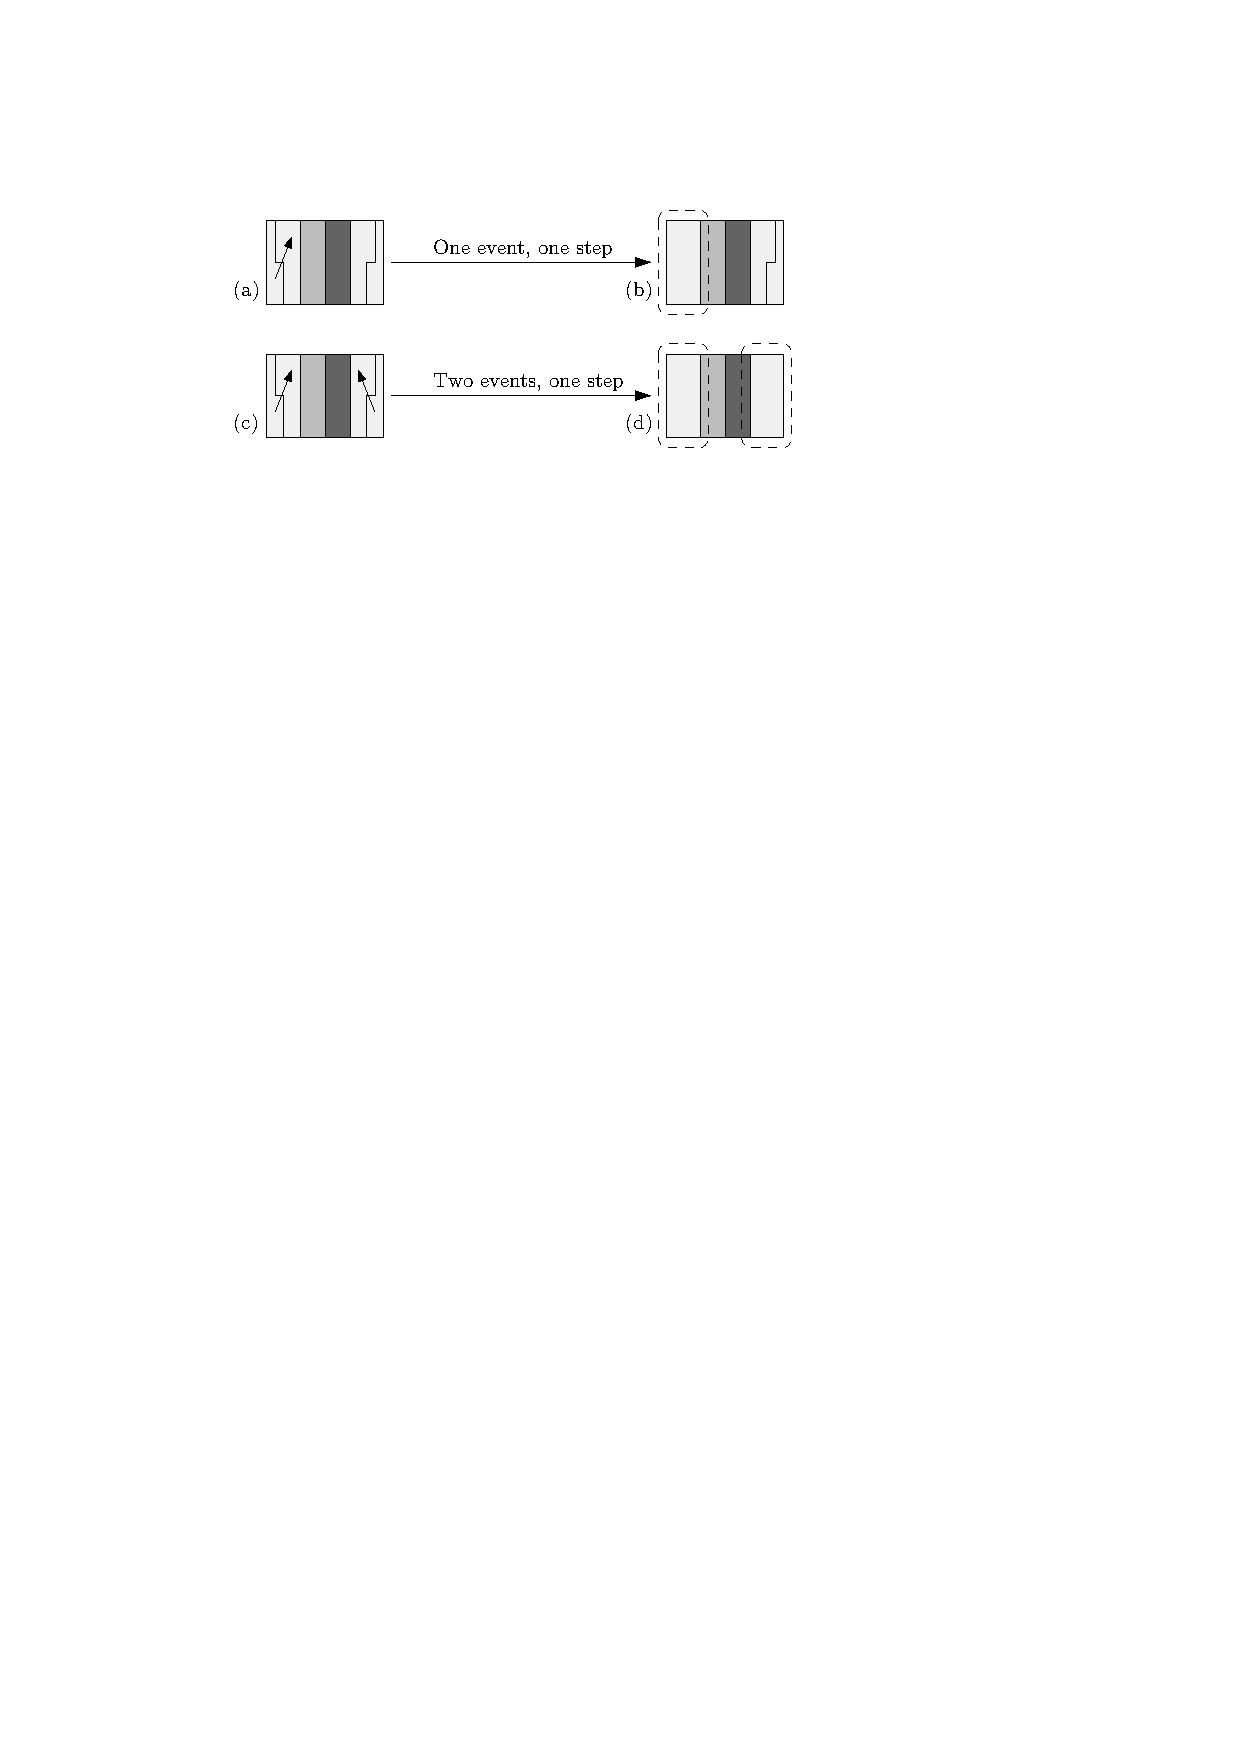
\includegraphics[page=1]{greedy_algorithm}
\caption{Illustration of the merging event and the merging step. 
Each path shows a merging step. 
A merging step consists of one or more merging events.}
\label{fig:event_and_step}
\end{figure}


We require that 
all the pairs of parcels involved in the merging events of a step 
do not have any common neighbors, 
which makes the merging events independent from each other.
There are two benefits of this independency.
First, it is easy to maintain the topology of the map.
When a pair of parcels have been merged, 
we must update the adjacent parcels in order to maintain the topology.
If an adjacent parcel is involved in another merging event,
then it will be complicated to update the parcel for the two merging events.
Second, users can more easily understand the events 
than merging several parcels into a single one,
where the latter is a traditional way of merging.
In order to realize the requirement, 
we block the neighbors of the selected parcels of merging events in a step
(see \fig\ref{fig:blocked_polygons}).
First, the adjacent parcels are blocked.
Second, the neighbors
of the adjacent parcels are blocked (see \fig\ref{fig:blocked_polygons}a).
When searching for another merging event for the step, 
we select the least important parcel and its most compatible neighbor
from the free parcels (see \fig\ref{fig:blocked_polygons}b);
if the most compatible neighbor is not free,
we block the the least important parcel 
and move to the next least important parcel.

\begin{figure}[tb]
\centering
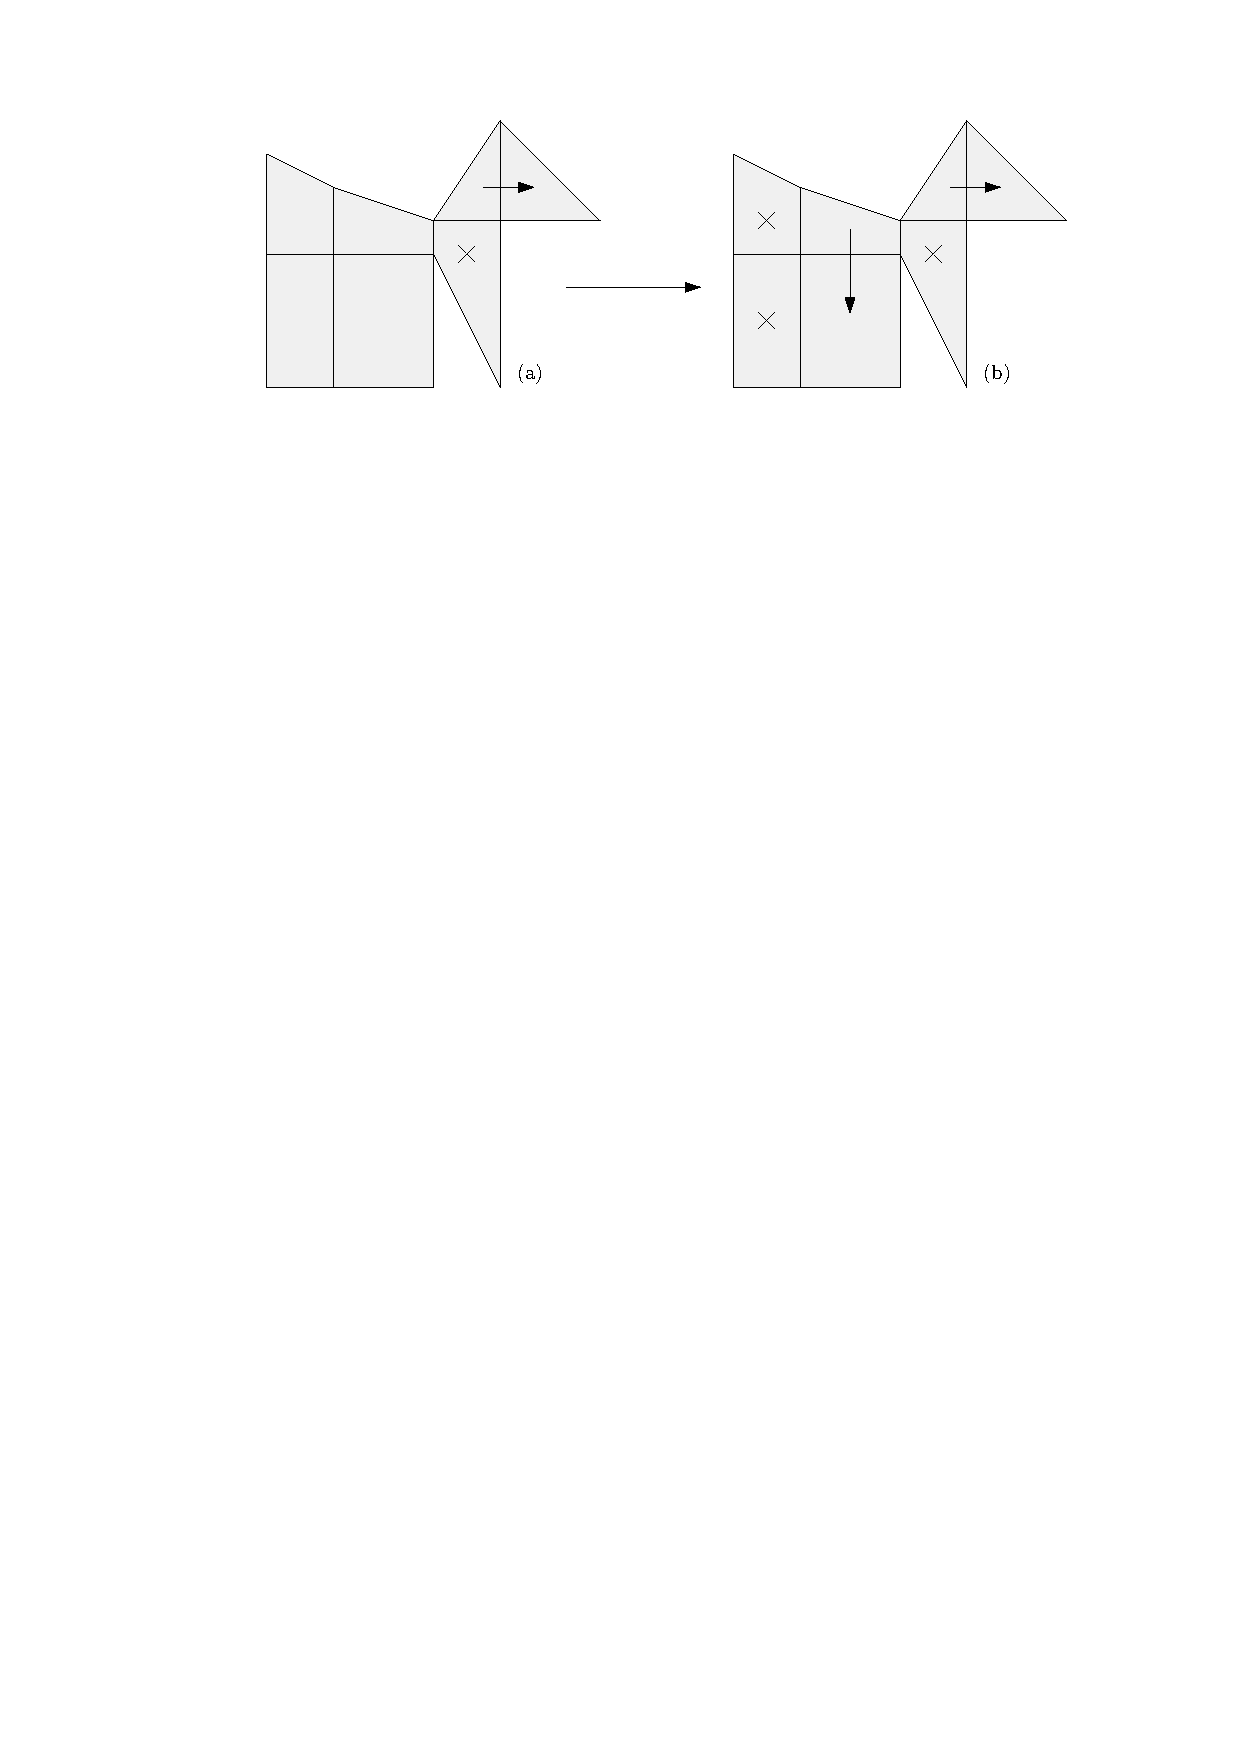
\includegraphics[]{blocked_polygons}
\caption{(a) From all the free parcels,
a least important one (marked by the small circle) is selected to merge into
its most compatible neighbor (marked by the larger circle).
Then the surrounding parcels are blocked (marked by the crosses).
(b) In order to find parallel merging events, 
a least important parcel from the remaining free parcels
is selected to merge with the most compatible neighbor,
and the surrounding parcels are blocked.
}
\label{fig:blocked_polygons}
\end{figure}



\subsection{A Greedy Algorithm}
\label{sec:greedy_algo}


We use a greedy algorithm to find the merging events of each step.
The algorithm selects the least important parcel and merge it with
the most compatible neighbor (that shares boundary).
There are many ways of defining the most compatible neighbor.
For example, \citet{Cheng2006} proposed three ways, i.e.,
the neighbor has the largest size, 
shares longest boundary with the least important parcel,
or is closest to the least important parcel in land-cover type. 
\citet{Peng2017AStar} proposed that 
the neighbor should have a close land-cover type
to the least important parcel
and the combination of the two parcels should be compact;
they defined the type distance based on a binary tree
according to the code of each land-cover type.

In this paper, we currently consider the most compatible neighbor
as the one shares the longest common boundary with the smallest parcel.
The greedy algorithm uses the two parcels for a merging event
and blocks the surrounding parcel (see \fig\ref{fig:blocked_polygons}a).
From the unblocked parcels, the algorithm finds another pair of parcels
for another merging event
(see \fig\ref{fig:blocked_polygons}b).
This finding process is iterated 
until a certain number of merging events have been found 
(e.g., 5\% of the number of parcels at the given stage), 
or there is no available pair of parcels for merging event anymore.
Up to this point, finding merging events for a step is finished,
and the parcels are merged in parallel.
Then the blocked parcels are released, 
and the finding of candidates for the next step starts.



%From the ordered sequence of the events, 
%we pick one by one if the later one will not 
%conflict with any of the previous events.
%
%We show how to find merging events for an merging step.
%We save all the adjacencies in a dictionary, say, $D_\mathrm{adj}$.
%We save all the neighbors of the involved patches of the selected events 
%in another dictionary, say, $D_\mathrm{nbr}$.
%For an event, we check if the adjacency of the two patches 
%exists in $D_\mathrm{adj}$.
%If so, and if no neighbor of the two patches exists in $D_\mathrm{nbr}$,
%then we add this event to the current merging step;
%otherwise, we skip this event for now.
%When we add this event, we also add all the neighbors of the two patches
%into dictionary $D_\mathrm{nbr}$.
%
%Two events conflict if they share a neighbor.

\subsection{Integrating the parallel events into the tGAP}

\citet[\fig5.9b]{Meijers2011Thesis} designed a table 
to record the face information of a tGAP.
The table contains columns \emph{face\_id}, 
\emph{imp\_low}, \emph{imp\_high}, \emph{imp\_own},
\emph{feature\_class\_id}, \emph{area}, and \emph{bbox}.
We add columns \emph{step\_low} and \emph{step\_high} into the table, 
which make it easy to see when a face should appear or disappear 
(see \tbls\ref{tab:face_tgap} and~\ref{tab:face_tgap_parallel},
where some columns are hidden).
That is, when the merging step arrives at the step\_low of a face,
then the face should appear;
when the merging step arrives at the step\_high of a face,
then the face should disappear;

When switching from merging one pair at each step 
(sequence~I of \fig\ref{fig:face_tgap})
to merging parallelly (sequence~II of \fig\ref{fig:face_tgap}),
we see that the step\_high values of faces~1 and~2 change from~1 to~2
(see \tbl\ref{tab:face_tgap_parallel}, the new values are in bold).
We also see that the step\_low value of faces~7 changes from~1 to~2
(see \tbl\ref{tab:face_tgap_parallel}).

\textbf{explain the start step!!!}
When we merge a pair of parcels by expanding one over the other one,
we must know when we start the expansion.
A simple way is to add a column, say, \emph{step\_expand} 
into the face table to record the step of starting expansion,
but this will increase the size of the face table.
To keep the face table compact,
we compute value step\_expand on the fly by
$$
step\_expand_i = 
$$


According to \tbl\ref{tab:face_tgap}, 
face~1 and face~2 are merged from step~0 to step~1,
which is before the merging of face~5 and face~6 from step~1 to step~2.
According to \tbl\ref{tab:face_tgap_parallel}, 
the merging of face~1 and face~2 and the merging of face~5 and face~6
happen parallelly from step~0 to step~2.

Then, the space-scale cube will be built 
according to the records of \tbl\ref{tab:face_tgap_parallel}.


\begin{figure}[tb]
\centering
\includegraphics[page=2]{greedy_algorithm}
\caption{Merging one pair of parcels at each step (sequence~I), 
    and merging two pairs of parcels parallelly (sequence~II).}
\label{fig:face_tgap}
\vspace{6mm} %for some reason, the space below the caption is not enough
%
%
%
\parbox{.49\linewidth}{
\captionof{table}{Face table of merging sequence~I 
    of \fig\ref{fig:face_tgap}.
}
\label{tab:face_tgap}
\centering
\begin{tabular}{ccc}
\hline
face\_id &   step\_low   & step\_high    \\ \hline
1       &     0         &     1          \\
2       &     0         &     1          \\
3       &     0         &     3          \\ 
4       &     0         &     3          \\
5       &     0         &     2          \\
6       &     0         &     2          \\         
7       &     1         &     3          \\
8       &     2         &     3          \\ \hline
\end{tabular}
}
%
%
\parbox{.49\linewidth}{
\captionof{table}{Face table of merging sequence~II 
    of \fig\ref{fig:face_tgap}.
}
\label{tab:face_tgap_parallel}
\centering
\begin{tabular}{ccc}
\hline
face\_id &   step\_low   & step\_high    \\ \hline
1       &     0         & \textbf{2}          \\
2       &     0         & \textbf{2}          \\
3       &     0         &     3          \\ 
4       &     0         &     3          \\
5       &     0         &     2          \\
6       &     0         &     2          \\         
7       &  \textbf{2}   &     3          \\
8       &     2         &     3          \\ \hline
\end{tabular}
}
\end{figure}


\subsection{Smooth Merging}
\label{sec:smooth_merging}

In order to provide smooth zooming of merging
so that map users easily understand the changes,
we merge by gradually expanding a parcel over another parcel
(see \fig\ref{fig:smooth_merging}).
This expansion is based on slicing the space-scale cube shown in
\fig\ref{fig:smooth_merging_two_rectangles}.
For example, \figs\ref{fig:smooth_merging}a,
\ref{fig:smooth_merging}b, and \ref{fig:smooth_merging}c
are respectively obtained from slicing the cube 
at the bottom, the middle, and the top.
The details of slicing a cube can be found in \citet{Meijers2020Web}.
The cube of \fig\ref{fig:smooth_merging_two_rectangles} was built 
based on the \emph{Eater} of \citet{Suba2014Merge}.
The Eater was used because it provides a solution 
for a parcel with any kind of shape, which is more robust than
\emph{Single flat plane} and \emph{Zipper} \citep{Suba2014Merge}.
Note that the common boundary of the two parcels disappears
very shortly after the expansion starts;
the common boundary exists only in \fig\ref{fig:smooth_merging}a but not in
\fig\ref{fig:smooth_merging}b,
\fig\ref{fig:smooth_merging}c, or
\fig\ref{fig:smooth_merging}d.


\begin{figure}[tb]
\centering
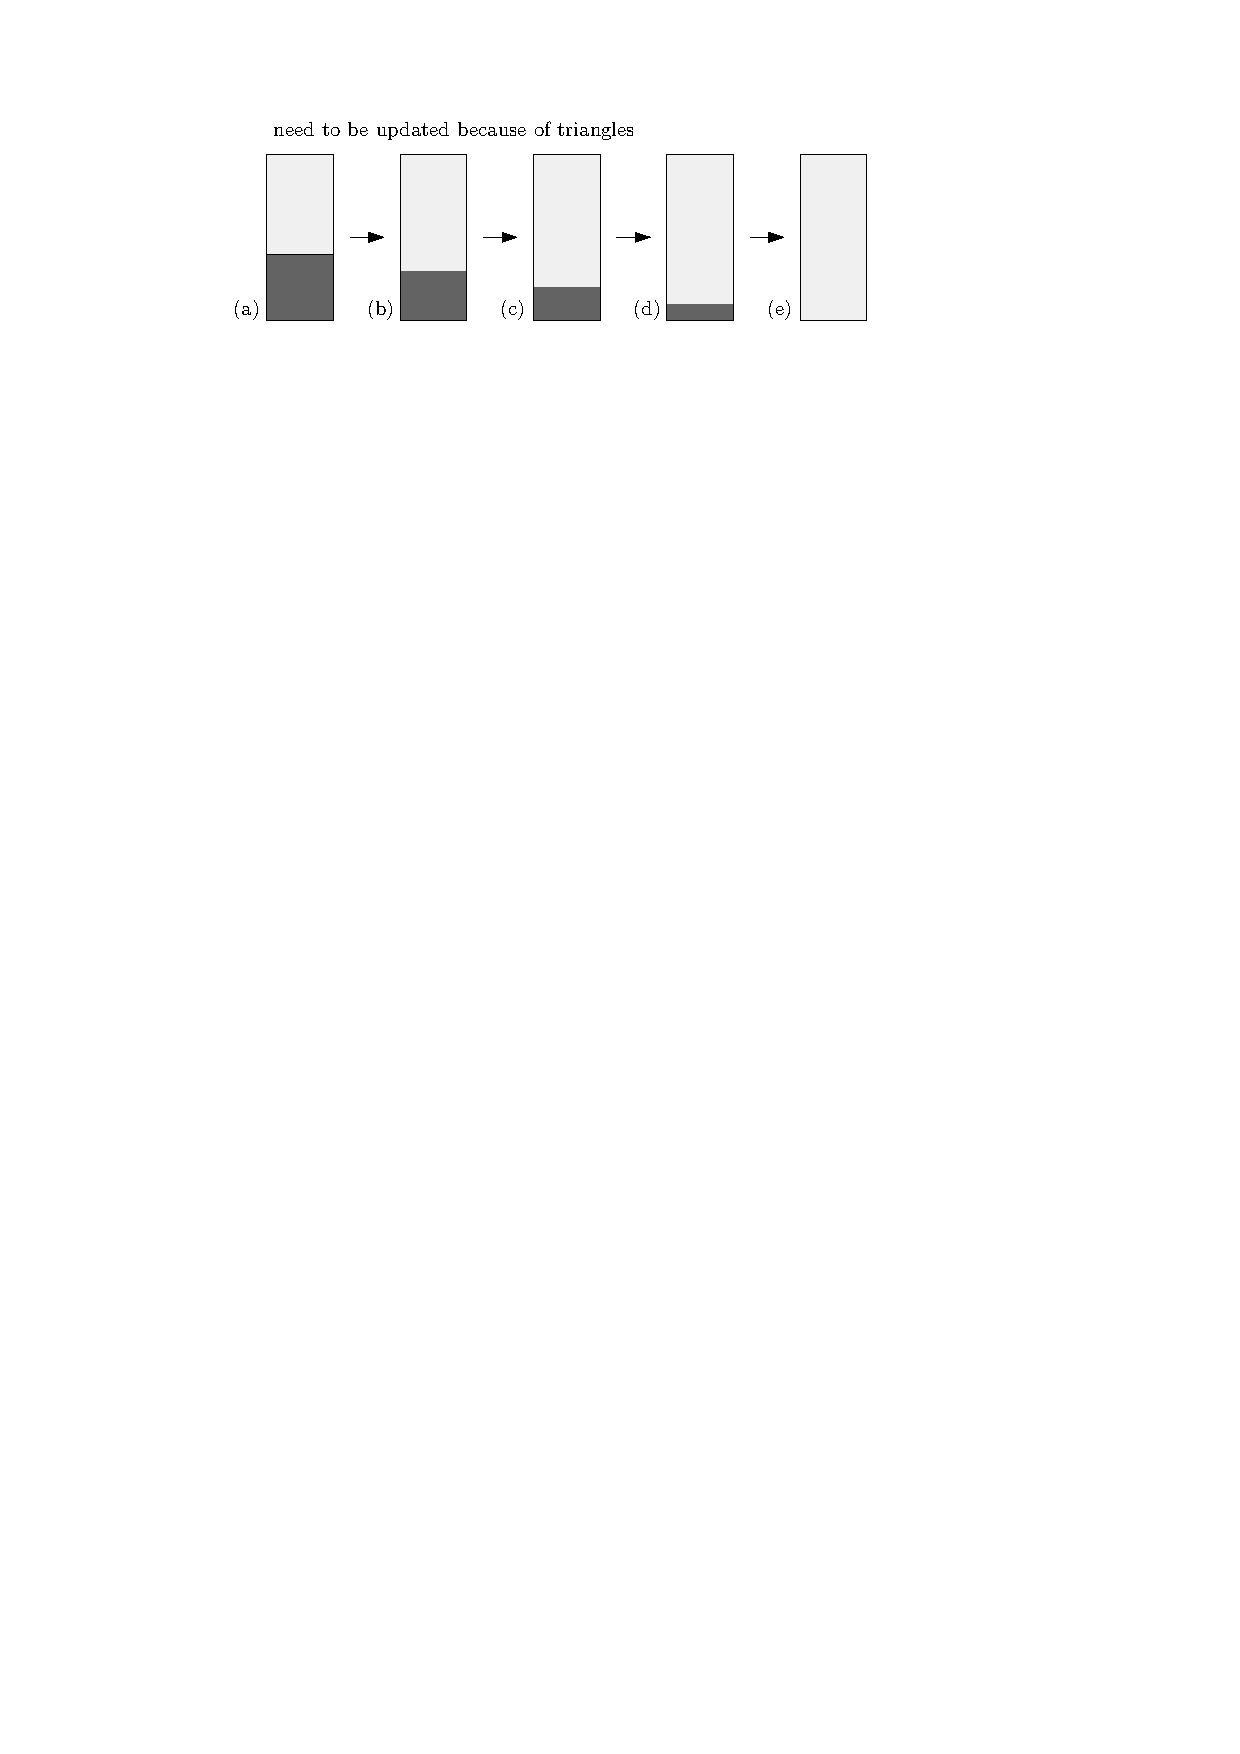
\includegraphics[page=1]{smooth_merging}
\caption{A smooth way of merging two parcels,
    where the larger parcel gradually expands over the smaller one.}
\label{fig:smooth_merging}
%
\vspace{6mm}
%
\centering
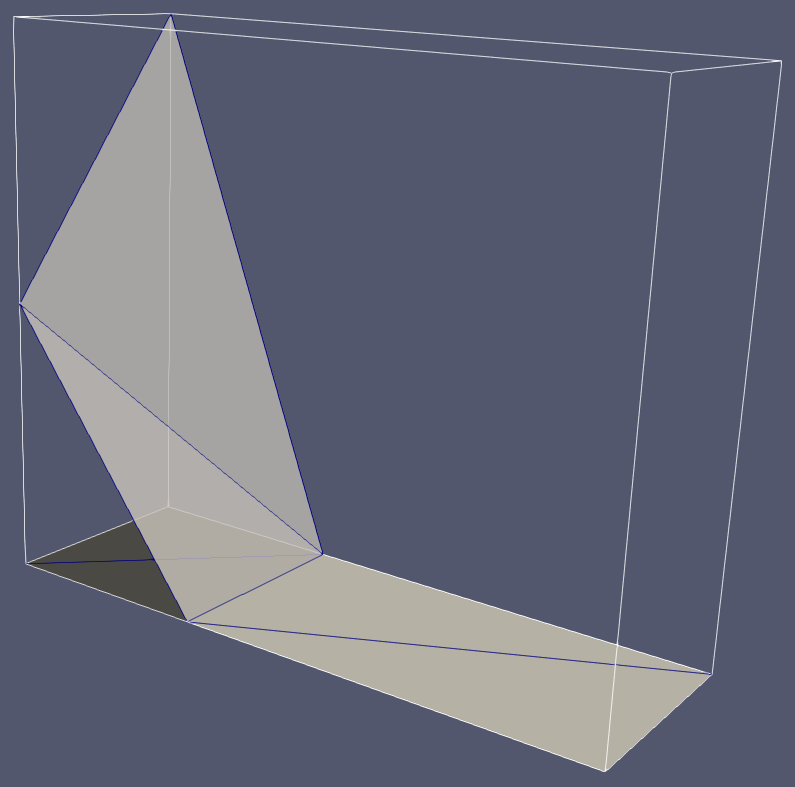
\includegraphics[scale=0.2]{smooth_merging_two_rectangles}
\caption{The space-scale cube for the merging 
    in \fig\ref{fig:smooth_merging}.
    This figure is made by visualizing the content of an obj file in 
    ParaView 5.6.0.}
\label{fig:smooth_merging_two_rectangles}
\end{figure}


%\begin{figure}[tb]
%\centering
%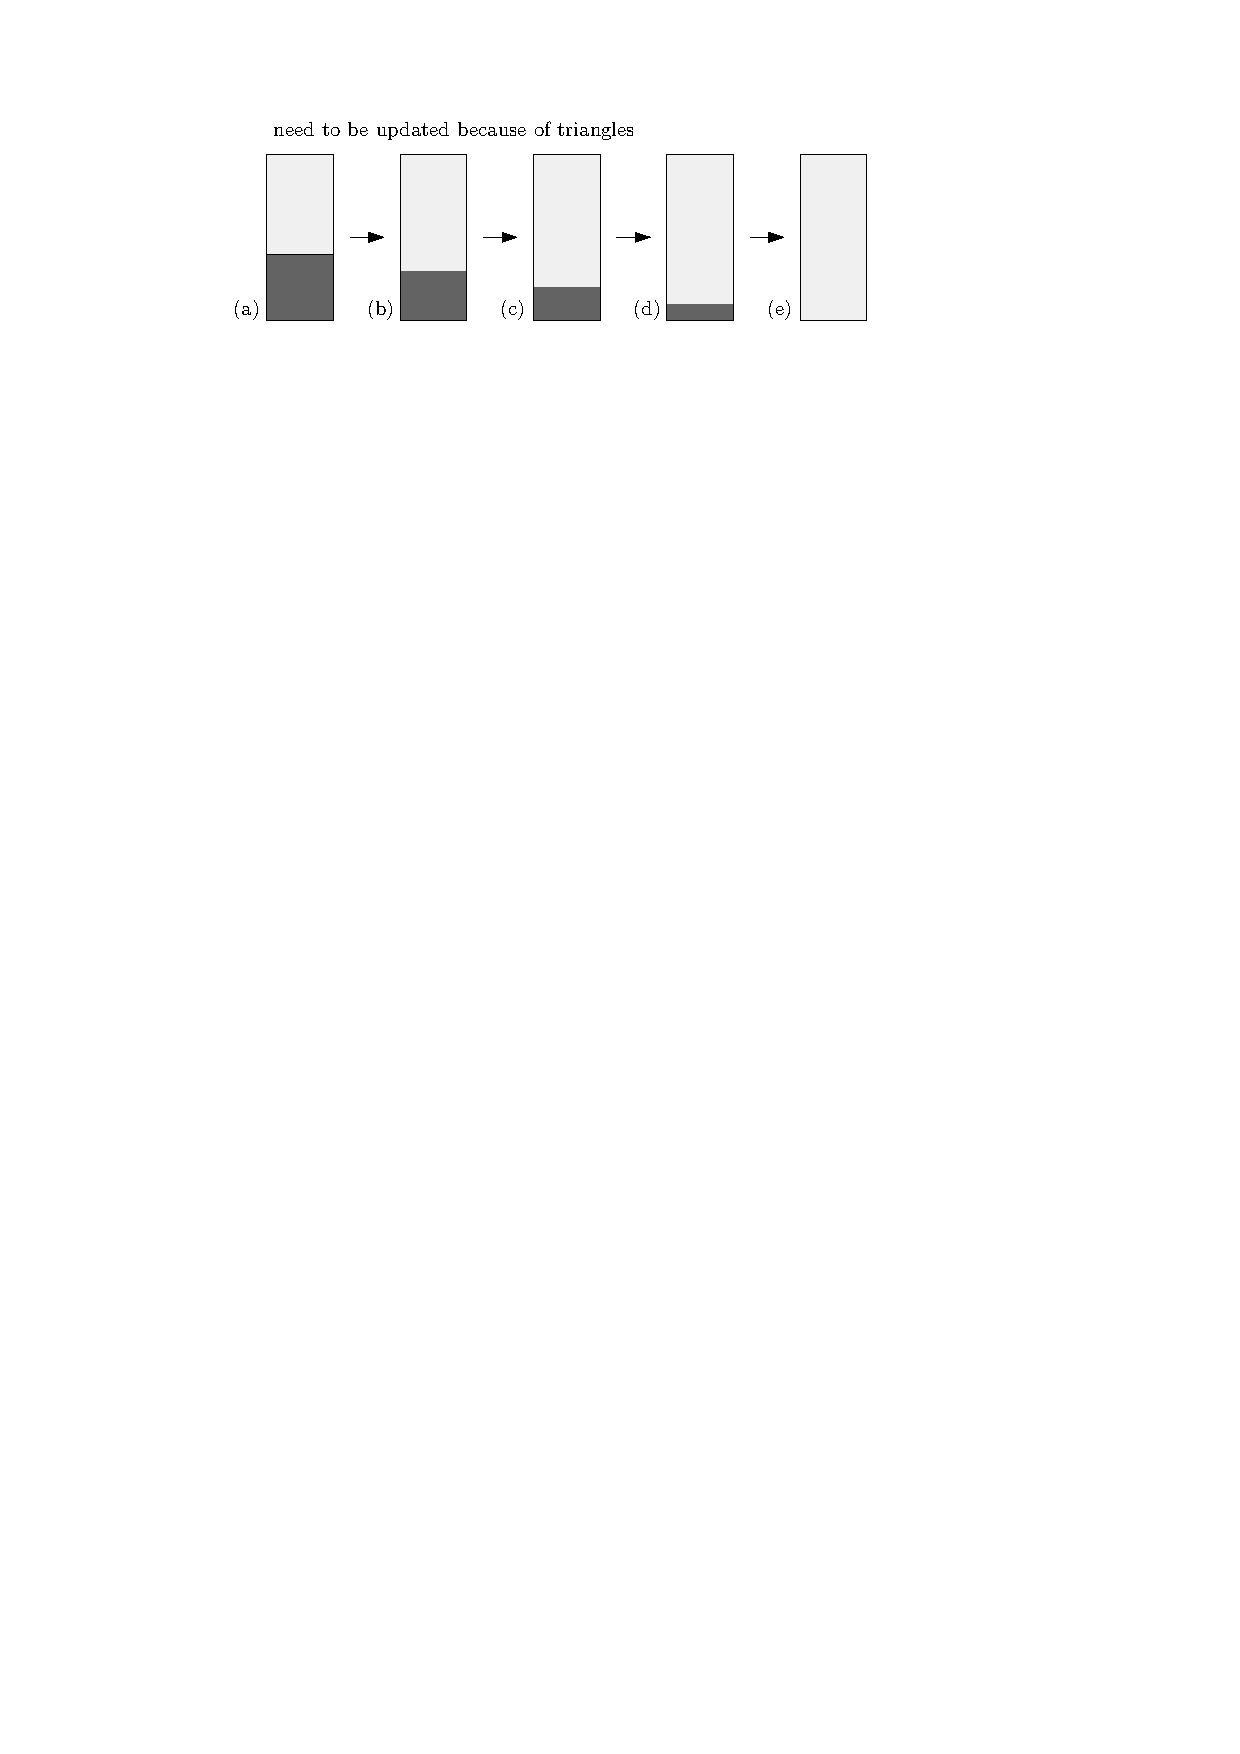
\includegraphics[page=1]{smooth_merging}
%\caption{pass.}
%\label{fig:smooth_merging}
%\end{figure}

%\begin{figure}[tb]
%\centering
%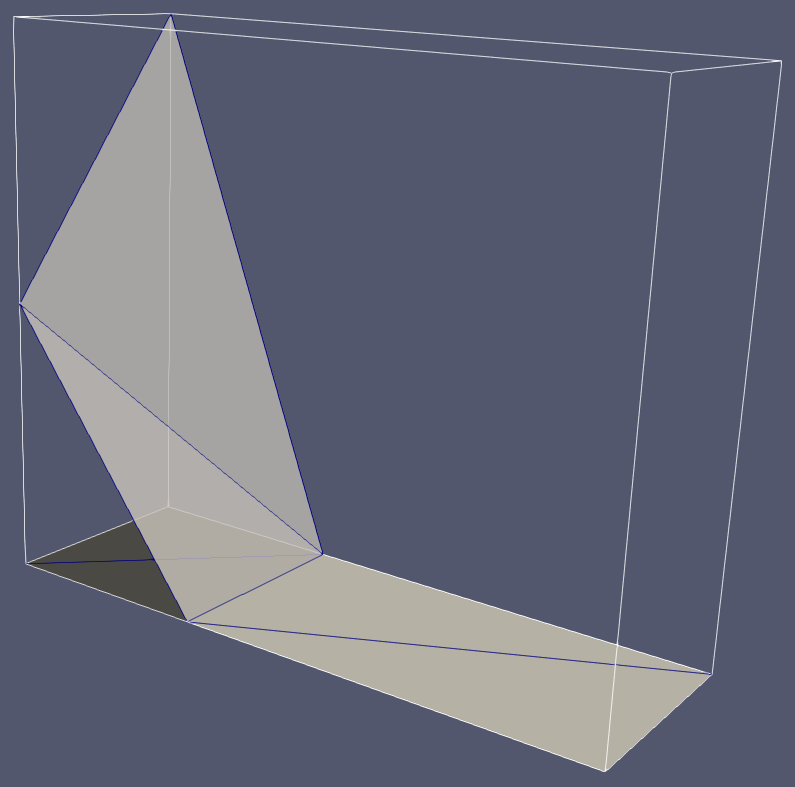
\includegraphics[scale=0.2]{smooth_merging_two_rectangles}
%\caption{pass.}
%\label{fig:smooth_merging_two_rectangles}
%\end{figure}

\subsection{Snapping to Certain Steps}
\label{sec:snap}

For a zooming action
(that is, slicing the SSC with a horizontal plane), 
we always snap the map to a certain step
so that users will not see a merging operation stops half-way
and will not see transition artifact (such as slivers or blended colors).
In order to do that, we store the information of
merging events and merging steps into 
a JSON file (JavaScript Object Notation File).
For example, given a base map of land-cover parcels,
we want to parallelly merge these parcels to generate a map
at a smaller scale.
If the parallel-event numbers of the merging steps are 
$60, 60, 60, 60, 60, 50, 50, 50, 30, 35$, and $35$ ($11$ steps in total),
then the content of the JSON file is
$$
\{\textrm{"eventnum\_repetition"}: [[60, 5], [50, 3], [30, 1], [35, 2]]\},
$$
where each pair of numbers in the inner square brackets 
represent the event number and the repeat times.


When a user opens our web map,
the JSON file will be transferred to the client.
The content of the file will be unpacked as 
a list of numbers~$L_\mathrm{event} = 
[0, 60, 120, 180, 240, 300, 350, 400, 450, 480, 515, 550]$.
According to how much a user has zoomed,
a scale, say $1:S_t$, can be computed.
According to \citet{Huang2016Webmap},
the number of merging events that should be processed can be computed by
\begin{equation}
\label{eq:E_t}
E_t = N_b \left(1-\frac{S^2_b}{S^2_t}\right),
\end{equation}
where parameter~$S_b$ is the scale denominator of the base map,
and parameter~$N_b$ is the number of parcels on the base map.
In our example regarding to list~$L_\mathrm{event}$,
if event number~$E_t \le 0$, the base map should be presented;
if $E_t \ge 550$, the map with all the merging events having been processed
should be presented.
Otherwise, if $0<E_t < 550$, we snap event number~$E_t$ 
to the closest value in list~$L_\mathrm{event}$,
which is marked by $E_{t,\mathrm{snap}}$.
The scale denominator corresponding to event number~$E_{t,\mathrm{snap}}$
can be computed by 
\begin{equation}
\label{eq:S_t_snap}
S_{t,\mathrm{snap}} = S_b \sqrt{\frac{N_b}{N_b-E_{t,\mathrm{snap}}}}.
\end{equation}
Note that \eq\ref{eq:S_t_snap} is an inverse function of \eq\ref{eq:E_t}.
At the end of the zooming action, 
the map will stop at scale~$1:S_{t,\mathrm{snap}}$.


%\subsection{Line simplification (smoothly moving vertices for the SSC)}


\section{Case Study}
\label{sec:case_study}

We have used the ``Eater'' of \citet{Suba2014Merge},
implemented in Python, 
to generate the elements of the SSC \citep{vanOosterom2014tGAPSSC} 
and saved these elements in an OBJ file\footnote{%
Wavefront .obj file:
\url{https://en.wikipedia.org/wiki/Wavefront_.obj_file},
accessed: Jan 14, 2020.}.
%
The OBJ file will be sent to the client 
when a user visits our website to access the map.
On the client side,
the content of the OBJ file is processed
by a prototype implemented in JavaScript.
The processed content and some code for WebGL (Web Graphics Library)
are submitted to GPU to display the map of smooth zoom.

The dataset used in this case study is a subset of TOP10NL\footnote{%
More information about TOP10NL can be found at
\url{https://zakelijk.kadaster.nl/-/topnl},
accessed: Jan 14, 2020.},
produced by Kadaster.
%
\figs\ref{fig:data}a and~\ref{fig:data}c show the map and the legend\footnote{%
More details about the type code and the rendering formula can be found at
\url{http://register.geostandaarden.nl/visualisatie/top10nl/1.2.0/BRT_TOP10NL_1.2_beschrijving_visualisatie.xlsx},
accessed: Jan 15, 2020.}.
%
Because the base scale is $1:10{,}000$, 
we have~$S_b = 10{,}000$ for \eq\ref{eq:S_t_snap}.
The maximum value of event number~$E_{t,\mathrm{snap}}$ is~$13{,}237$
as there are in total~$13{,}238$ parcels.
When we zoom out far enough 
so that~$E_{t,\mathrm{snap}}$ reaches its maximum value,
the scale denominator will arrive at~$1{,}150{,}565$
according to \eq\ref{eq:S_t_snap}.
At that moment, all the parcels are merged into one single parcel
(see \figs\ref{fig:data}b).


\begin{figure}[tb]
\centering
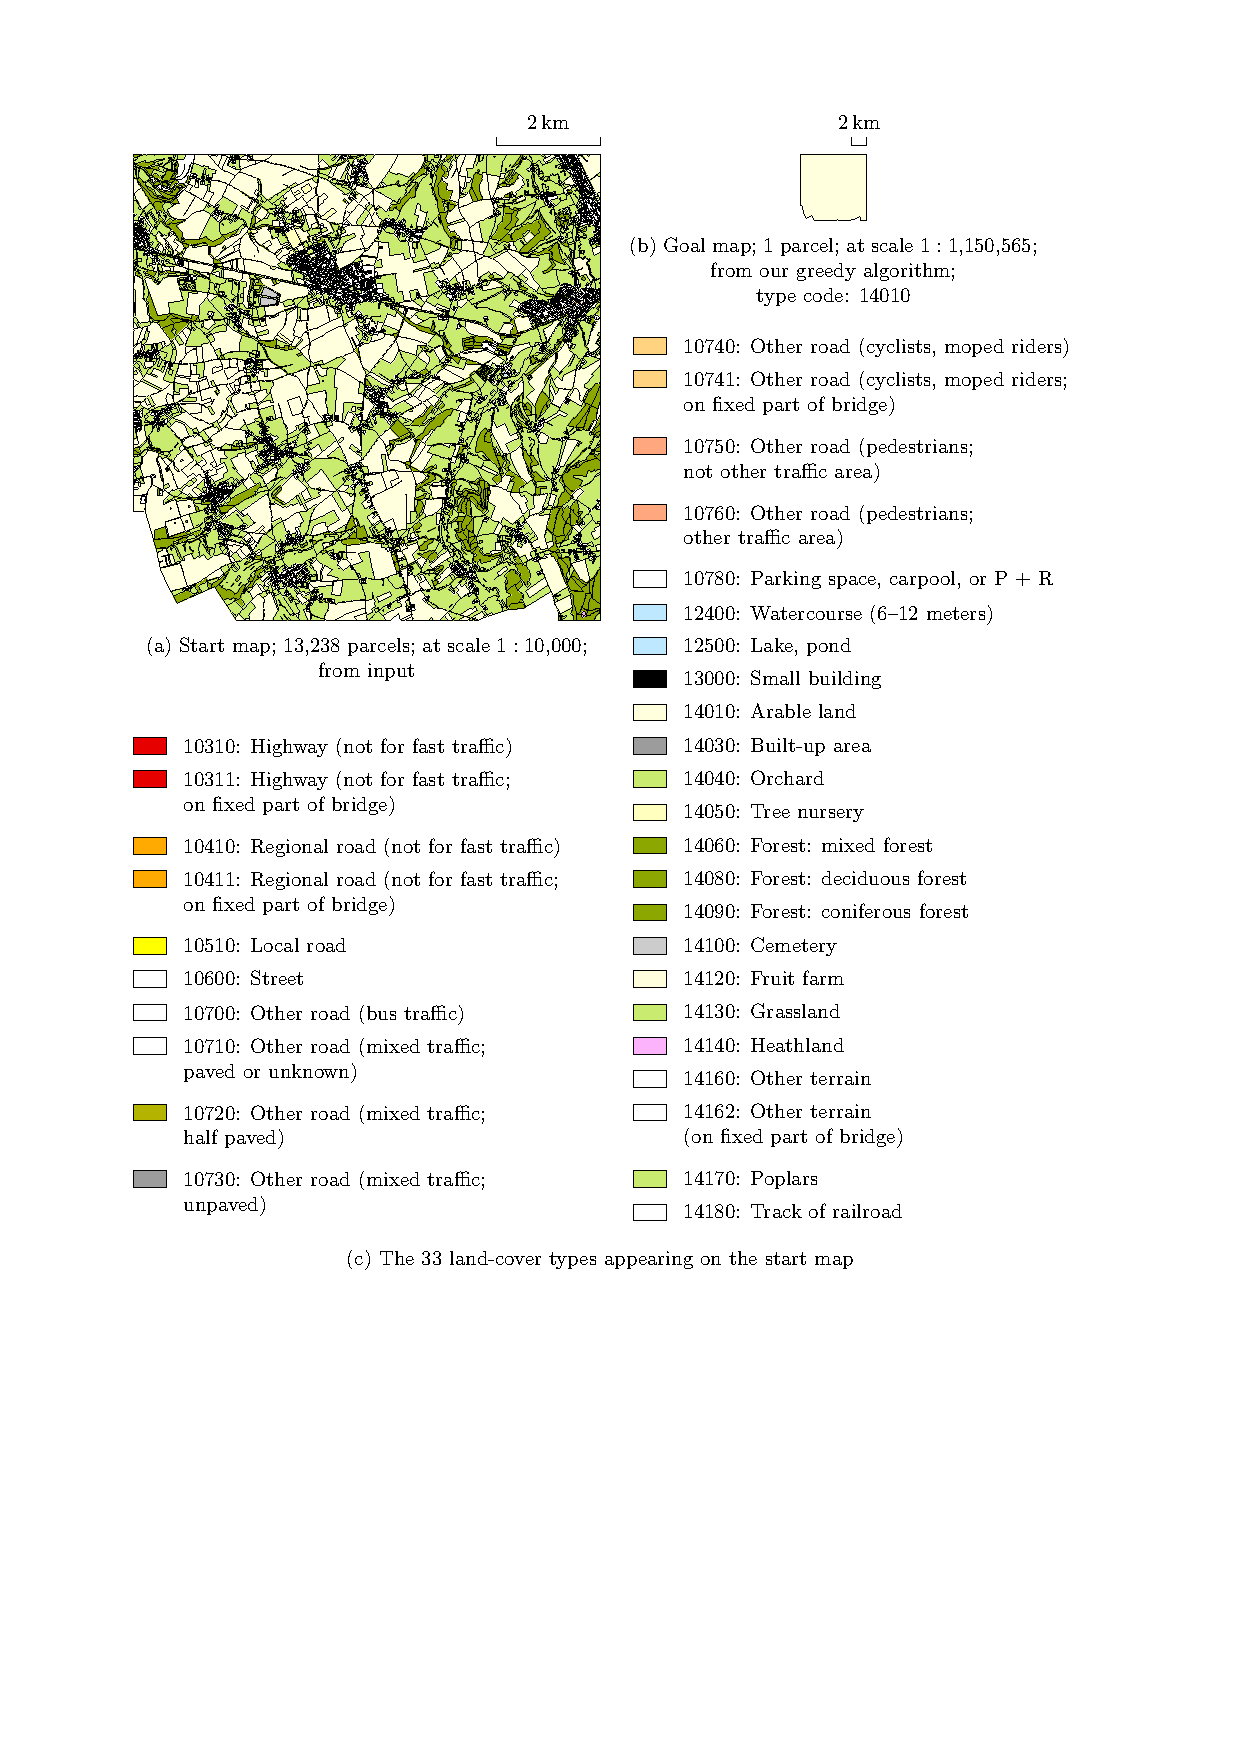
\includegraphics[page=1]{data}
\caption{The dataset represents the place 
    to the southeast of Maastricht, Limburg, The Netherlands.}
\label{fig:data}
\end{figure}


Parameter~$N_\mathrm{parallel}$, 
the maximum number of parallel events mentioned in \sect\ref{sec:greedy_algo},
was set to~$200$.
The content of the JSON file (see \sect\ref{sec:snap}) is 
\makeatletter
\def\verbatim@font{\normalfont\rmfamily}
\makeatother
\begin{verbatim}
{"eventnum_repetition": [[200, 46], [191, 1], [183, 1], [178, 1], [167, 1], [165, 1], [146, 1], [145, 1], [136, 1], 
[135, 1], [127, 1], [124, 1], [108, 1], [103, 1], [107, 1], [96, 1], [95, 1], [87, 1], [82, 1], [81, 1], [82, 1],  [78, 1], 
[75, 1], [69, 1], [66, 1], [61, 1], [56, 1], [57, 1], [54, 1], [48, 1], [47, 1], [49, 1], [44, 1], [45, 1], [42, 1], [37, 1], [41, 1], 
[34, 1], [36, 1], [29, 1], [28, 1], [27, 1], [24, 1], [25, 1], [20, 2], [22, 1], [21, 1], [19, 3], [15, 1], [13, 1], [12, 1], [13, 1], 
[12, 1], [11, 1], [9, 1], [12, 3], [9, 1], [10, 2], [9, 1], [7, 1], [6, 1], [7, 2], [5, 2], [6, 4], [5, 3], [4, 2], [3, 7], [2, 4], [1, 2], 
[2, 1], [1, 11]]}.
\end{verbatim}
There are~$150$ steps in total, 
which can be computed by summing up the second values of all the pairs.



The number of times that we compromised.
Because some parcels are blocked during finding merging events, 
the least important parcel selected for an merging event 
is not the real least important parcel 
among all the parcels at that step. 
This situation happens $XXX$ times in our data.
For the same reason, 
we cannot always use the most compatible adjacent parcel,
which happens $XXX$ times.






\section{Concluding Remarks}
\label{sec:concluding_remarks}

\subsection{Conclusion}
This paper proposed a greedy algorithm to find parallel events of 
merging land-cover parcels.
Then, we integrated the parallel events into the SSC. 
On the client side, web maps are generated by slicing the SSC
based on the method of \citet{Meijers2020Web}.
To avoid half-way merging, we require the merging animation 
to stop at complete steps (which contain parallel events).
Our case study shows that 
our approach provides with more smooth transition for zooming.


\subsection{Future Work}



Our current event consists of only the merging operation,
it is also necessary to involve split operation
because sometimes a merging operation results in an unnatural parcel.
For example, it is weird to merge a long and thin parcel 
with one of the parcels that are along it
\citep[see][]{Haunert2008Skeleton}.
Therefore, such kind of long and thin parcels should be
split into several parts first.
We may integrate a split method based on the straight skeleton
\citep{Haunert2008Skeleton}
or the skeleton based on constrained Delaunay triangulation
\citep{Meijers2016Split}.
In order to apply appropriate generalization operators
for a certain scale,
we also need to extend and implement the framework 
to guide our generalization choices
\citep{Meijers2018Framework}.

To avoid clutter of vertices for zooming out, 
we also need to simplify the boundaries of the parcels.
\citet{Meijers2011LineSimp} proposed a method 
to simplify the boundaries parallelly. 
Moreover, their results are topologically safe . 
Another choice would be the method of \citet{ImaiIri1988},
which is able to minimize the number of vertices 
for a given error threshold.
One more choice would be to construct compatible triangulations 
\citep[see][\chap3]{Peng2019Thesis}
for the two levels of land-cover maps.
In the SSC, we could build some tilted walls 
to connect the two levels of compatible triangulations.
When we slice this SSC to animate a zooming action,
the boundaries of the parcels are morphed 
between a detailed representation and a coarse representation.
We can imagine that it is challenging to build the tilted walls.

evenly distribute the merging events for each step, 
network simplification

When we remove a triangle by slicing the SSC, 
we may want to keep three vertices of the triangle 
instead of making four vertices.
In this case, the polyhedron (with five faces) should have curly edges,
which is also known as a \emph{curved polyhedron}.
The slopes of curly edges need to be studied.

\sect\ref{sec:smooth_merging} shows our current solution of
gradually expanding a parcel over the other parcel.
In order to make the expansion even more smooth,
we would like to implement the way 
shown in \fig\ref{fig:smooth_merging_future}.

\begin{figure}[tb]
\centering
\includegraphics[page=2]{smooth_merging}
\caption{A smooth way of merging two parcels.
    The larger parcel expands over the smaller one.
    At the same time, 
    the smaller parcel gradually adapt to the color of the larger one,
    and the common boundary becomes thinner and thinner.}
\label{fig:smooth_merging_future}
\end{figure}

This paper used a greedy algorithm 
to find parallel merging events for each step.
Alternatively, it is also possible to find a sequence of merging steps,
where each step consists only one merging event, by some existing methods
(e.g., the greedy algorithm of \citet{vanOosterom2005}
or the \Astar algorithm of \citet[\chap2]{Peng2019Thesis}).
Then, we can reorganize some of the single-event merging steps 
to form some parallel-event merging steps.

This paper develops technique for smooth zooming based on parallel merging,
and we hope that it allows map users to follow the zooming more easily.
A future work is to investigate 
how much map users benefit from our technique.
We will conduct some usability tests based on the experience of
\citet[\sect6.7]{Suba2017Thesis} and \citet{Midtbo2007}.


%Some research questions are as follows.
%What aspects should we optimize 
%(e.g., minimizing the number of merging events or 
%assigning similar numbers of merging steps to each event)?
%What algorithm should we use 
%(e.g., dynamic programming, \Astar, or integer linear programming)?
%How much time is gained for users to observe the merging steps on the screen?
%How to store the parallel merging steps?









%%%%%%%%%%%%%%%%%%%%%%%%%%%%%%%%%%%%%%%%%%%
%\section{Patents}
%This section is not mandatory, but may be added if there are patents resulting from the work reported in this manuscript.
%
%%%%%%%%%%%%%%%%%%%%%%%%%%%%%%%%%%%%%%%%%%%
%\vspace{6pt} 
%
%%%%%%%%%%%%%%%%%%%%%%%%%%%%%%%%%%%%%%%%%%%
%%% optional
%%\supplementary{The following are available online at \linksupplementary{s1}, Figure S1: title, Table S1: title, Video S1: title.}
%
%% Only for the journal Methods and Protocols:
%% If you wish to submit a video article, please do so with any other supplementary material.
%% \supplementary{The following are available at \linksupplementary{s1}, Figure S1: title, Table S1: title, Video S1: title. A supporting video article is available at doi: link.}
%
%%%%%%%%%%%%%%%%%%%%%%%%%%%%%%%%%%%%%%%%%%%
%\authorcontributions{For research articles with several authors, a short paragraph specifying their individual contributions must be provided. The following statements should be used ``conceptualization, X.X. and Y.Y.; methodology, X.X.; software, X.X.; validation, X.X., Y.Y. and Z.Z.; formal analysis, X.X.; investigation, X.X.; resources, X.X.; data curation, X.X.; writing--original draft preparation, X.X.; writing--review and editing, X.X.; visualization, X.X.; supervision, X.X.; project administration, X.X.; funding acquisition, Y.Y.'', please turn to the  \href{http://img.mdpi.org/data/contributor-role-instruction.pdf}{CRediT taxonomy} for the term explanation. Authorship must be limited to those who have contributed substantially to the work reported.}
%
%%%%%%%%%%%%%%%%%%%%%%%%%%%%%%%%%%%%%%%%%%%
%\funding{Please add: ``This research received no external funding'' or ``This research was funded by NAME OF FUNDER grant number XXX.'' and  and ``The APC was funded by XXX''. Check carefully that the details given are accurate and use the standard spelling of funding agency names at \url{https://search.crossref.org/funding}, any errors may affect your future funding.}
%
%%%%%%%%%%%%%%%%%%%%%%%%%%%%%%%%%%%%%%%%%%%
%\acknowledgments{In this section you can acknowledge any support given which is not covered by the author contribution or funding sections. This may include administrative and technical support, or donations in kind (e.g., materials used for experiments).}
%
%%%%%%%%%%%%%%%%%%%%%%%%%%%%%%%%%%%%%%%%%%%
%\conflictsofinterest{Declare conflicts of interest or state ``The authors declare no conflict of interest.'' Authors must identify and declare any personal circumstances or interest that may be perceived as inappropriately influencing the representation or interpretation of reported research results. Any role of the funders in the design of the study; in the collection, analyses or interpretation of data; in the writing of the manuscript, or in the decision to publish the results must be declared in this section. If there is no role, please state ``The funders had no role in the design of the study; in the collection, analyses, or interpretation of data; in the writing of the manuscript, or in the decision to publish the results''.} 
%
%%%%%%%%%%%%%%%%%%%%%%%%%%%%%%%%%%%%%%%%%%%
%%% optional
%\abbreviations{The following abbreviations are used in this manuscript:\\
%
%\noindent 
%\begin{tabular}{@{}ll}
%MDPI & Multidisciplinary Digital Publishing Institute\\
%DOAJ & Directory of open access journals\\
%TLA & Three letter acronym\\
%LD & linear dichroism
%\end{tabular}}
%
%%%%%%%%%%%%%%%%%%%%%%%%%%%%%%%%%%%%%%%%%%%
%%% optional
%\appendixtitles{no} %Leave argument "no" if all appendix headings stay EMPTY (then no dot is printed after "Appendix A"). If the appendix sections contain a heading then change the argument to "yes".
%\appendix
%\section{}
%\unskip
%\subsection{}
%The appendix is an optional section that can contain details and data supplemental to the main text. For example, explanations of experimental details that would disrupt the flow of the main text, but nonetheless remain crucial to understanding and reproducing the research shown; figures of replicates for experiments of which representative data is shown in the main text can be added here if brief, or as Supplementary data. Mathematical proofs of results not central to the paper can be added as an appendix.
%
%\section{}
%All appendix sections must be cited in the main text. In the appendixes, Figures, Tables, etc. should be labeled starting with `A', e.g., Figure A1, Figure A2, etc. 

%%%%%%%%%%%%%%%%%%%%%%%%%%%%%%%%%%%%%%%%%%
% Citations and References in Supplementary files are permitted provided that they also appear in the reference list here. 

%=====================================
% References, variant A: internal bibliography
%=====================================
%\reftitle{References}
%\begin{thebibliography}{999}
%% Reference 1
%\bibitem[Author1(year)]{ref-journal}
%Author1, T. The title of the cited article. {\em Journal Abbreviation} {\bf 2008}, {\em 10}, 142--149.
%% Reference 2
%\bibitem[Author2(year)]{ref-book}
%Author2, L. The title of the cited contribution. In {\em The Book Title}; Editor1, F., Editor2, A., Eds.; Publishing House: City, Country, 2007; pp. 32--58.
%\end{thebibliography}
\bibliography{Reference/BibReference}

% The following MDPI journals use author-date citation: Arts, Econometrics, Economies, Genealogy, Humanities, IJFS, JRFM, Laws, Religions, Risks, Social Sciences. For those journals, please follow the formatting guidelines on http://www.mdpi.com/authors/references
% To cite two works by the same author: \citeauthor{ref-journal-1a} (\citeyear{ref-journal-1a}, \citeyear{ref-journal-1b}). This produces: Whittaker (1967, 1975)
% To cite two works by the same author with specific pages: \citeauthor{ref-journal-3a} (\citeyear{ref-journal-3a}, p. 328; \citeyear{ref-journal-3b}, p.475). This produces: Wong (1999, p. 328; 2000, p. 475)

%=====================================
% References, variant B: external bibliography
%=====================================
%\externalbibliography{yes}
%\bibliography{your_external_BibTeX_file}

%%%%%%%%%%%%%%%%%%%%%%%%%%%%%%%%%%%%%%%%%%
%% optional
%\sampleavailability{Samples of the compounds ...... are available from the authors.}

%% for journal Sci
%\reviewreports{\\
%Reviewer 1 comments and authors’ response\\
%Reviewer 2 comments and authors’ response\\
%Reviewer 3 comments and authors’ response
%}




%%%%%%%%%%%%%%%%%%%%%%%%%%%%%%%%%%%%%%%%%%
\end{document}

